\documentclass[tikz,border=10pt]{standalone}

\usetikzlibrary{arrows.meta,calc}

\begin{document}
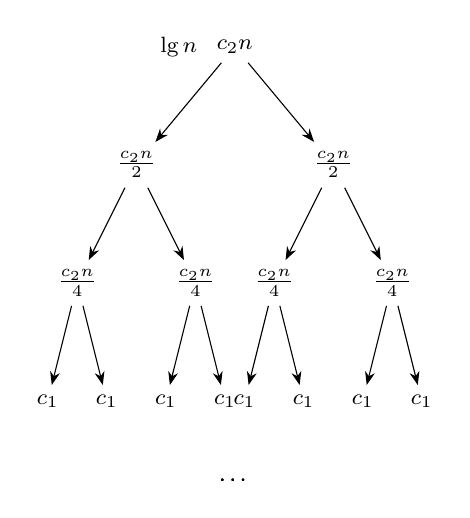
\begin{tikzpicture}[
  level distance=1.5cm,
  sibling distance=3.5cm,
  edge from parent/.style={draw, -{Stealth[]}},
  level 1/.style={sibling distance=2.5cm},
  level 2/.style={sibling distance=1.5cm},
  level 3/.style={sibling distance=0.75cm},
  every node/.style={font=\footnotesize},
  node distance=1cm and 1cm
]

% Root node
\node (root) {$c_2n$}
  child {node {$\frac{c_2n}{2}$}
    child {node {$\frac{c_2n}{4}$}
      child {node {$c_1$}}
      child {node {$c_1$}}
    }
    child {node {$\frac{c_2n}{4}$}
      child {node {$c_1$}}
      child {node {$c_1$}}
    }
  }
  child {node {$\frac{c_2n}{2}$}
    child {node {$\frac{c_2n}{4}$}
      child {node {$c_1$}}
      child {node {$c_1$}}
    }
    child {node {$\frac{c_2n}{4}$}
      child {node {$c_1$}}
      child {node {$c_1$}}
    }
  };

% Add dashed lines for continuation at the bottom
\foreach \i in {1,2,3,4} {
  \node at ($(root) + (0,-5.5)$) {\dots};
}

% Add additional labels
\node[left] at (root.west) {$\lg n$};
\end{tikzpicture}
\end{document}
